\chapter{Implementarea Alegria}
\newlength{\bulletwidth}\settowidth{\bulletwidth}{$\bullet$}
\newcommand{\mitem}{\setlength{\leftskip}{\leftmargin}\hspace*{-\labelsep}\hspace*{-\bulletwidth}$\bullet$\hspace*{\labelsep}}
\newcommand{\mend}{\setlength{\leftskip}{0cm}}
\section{Interfaţa Web}
\begin{wrapfigure}{r}{0.35\textwidth}
	\centering
	\captionsetup{justification=centering}
	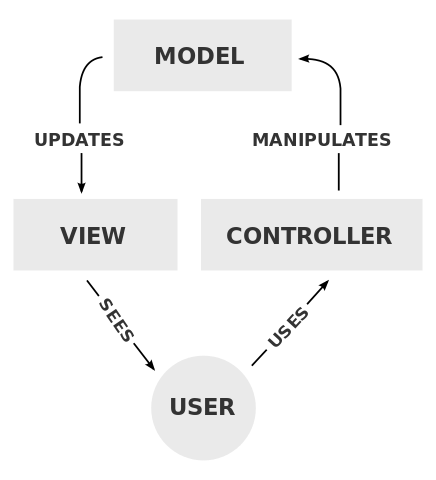
\includegraphics[width=0.35\textwidth]{mvcPattern}
	\caption{Colaborarea intre componentele MVC}
\end{wrapfigure}
Alegria a fost implementata cu ajutorul platformei \textbf{Spring Boot} \autocite{SpringBoot}. Platforma a fost aleasa pentru stabilitatea ei excepţională, fiind bazata pe Spring Framework care sta la baza unora din cele mai mari aplicaţii existente\autocite{springUseCase}, dar si pentru uşurinţa prin care o aplicaţie poate fi compusa din elemente funcţionale, abstractizând peste nivelele de jos a programului, permiţând alocarea timpului pe logica aplicaţiei, si nu pe implementarea platformei pe care aplicaţia sa ruleze. Un alt motiv pentru care platforma Spring a fost aleasa, este faptul ca suporta programarea orientată pe aspecte, si injecţia dependinţelor, permiţând scrierea de cod curat si uşor de testat.

Cum aplicaţia este bazata pe arhitectura MVC (model-view-controller)  aceasta a fost structurata in trei elemente separate: 

\mitem  \textbf{Interfaţa vizuala}: Realizata in \textbf{HTML5}, folosind motorul de templating Thymeleaf pe server si Bootstrap si JQuery in client pentru afişarea paginilor. Aceasta combinaţie permite realizarea de pagini cu un aspect modern, responsiv, care funcţionează atât pe ecranul mare al calculatorului, cat si pe display-ul mic al unui telefon.

\mitem  \textbf{Modele}: Reprezinta o reprezentare a entităţilor din baza de date in sistemul Alegria.

\mitem  \textbf{Controller-e}: Realizează legătura intre partea vizuala a aplicaţiei si entităţile din baza de date, asigurând atât metodele care "umplu" template-urile cu date, cat si implementarea interfeţei API care introduce si extrage date.

\mend

\subsection{Securitate}
Securitatea este un element de baza, atât pentru accesul la date, cat si pentru accesul la entităţi. Astfel, in implementare s-a folosit framework-ul \textbf{Spring Security} care usureaza management-ul securităţii, fiind puternic integrat si cu restul platformei Spring.
\begin{figure}[H]
	\centering
	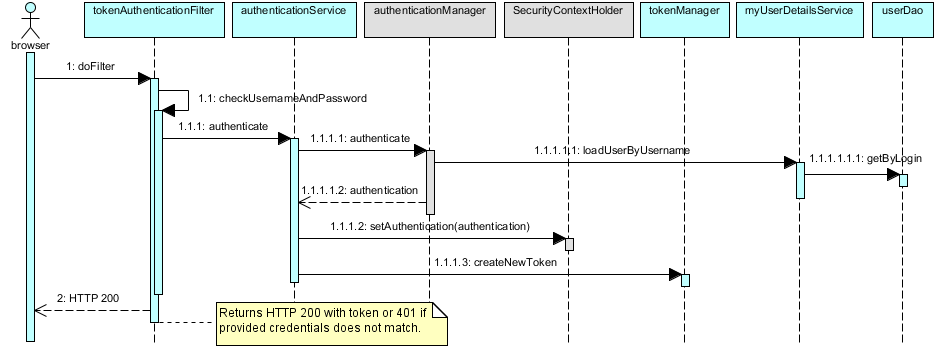
\includegraphics[width=1.35\textwidth, center]{loginUml}
	\caption{Procesul de autentificare in aplicaţie}
	\label{fig:loginUml}
\end{figure}
Pentru autentificare a accesa o resursa protejata, utilizatorul va folosi unul din doua mecanisme:
\begin{itemize}
	\item Autentificare securizata prin username si parola, aceste detalii fiind stocate in tabela \textit{application\_user}, unde parola a fost stocata dupa ce a fost trecuta printr-o funcţie criptografica de hashing. Aceasta metoda de autentificare este folosita pentru autentificarea utilizatorilor in interfaţă de management si monitorizare. Odată ce procesul a reuşit, un token unic va fi generat, iar request-urile următoare vor fi verificate pe baza procesului descris mai jos.
	\item Autentificare pe baza de token, folosita pentru securizarea API-ului, dar si in cazul in care un user s-a autentificat deja cu username si parola. Fiecare request trebuie sa aibă un token, fie într-un cookie, fie ca parametru in url.
\end{itemize}

Tot in scopuri de securitate, fiecare entitate care poate fi modificata menţine un istoric al tuturor modificărilor, împreuna cu utilizatorul cu care le-a efectuat, iar, pentru o dezvoltare ulterioara, accesul unui utilizator poate fi limitat doar la obiectele care au aceleaşi tag-uri ca si utilizatorul.
\subsection{Management}
\begin{figure}[H]
	\centering
	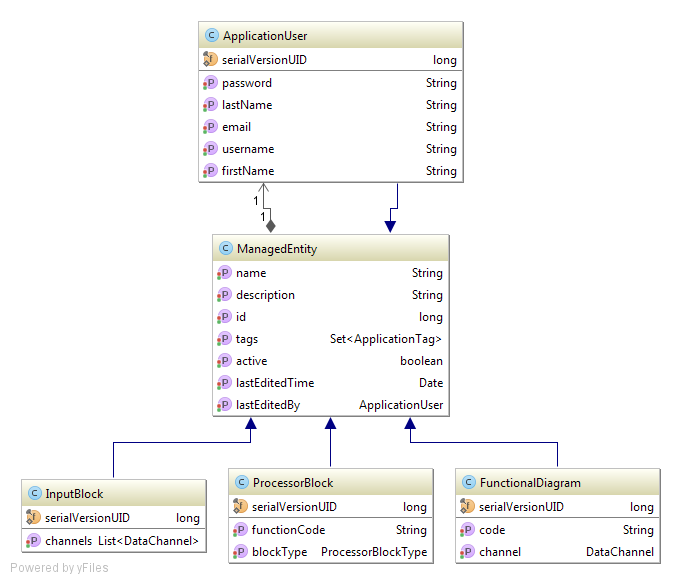
\includegraphics[width=\textwidth, center]{managedEntities}
	\captionsetup{justification=centering}
	\caption{Entităţile care sunt administrate de către utilizator si implementeaza \code{ManagedEntity}}
	\label{fig:managedEntities}
\end{figure}
Toate entităţile care implementeaza \code{ManagedEntity} permit apoi operaţii de adăugare, modificare si ştergere. Acest proces de administrare vizuala foloseşte următoarele resurse, iar un exemplu pentru management-ul :
\begin{itemize}
	\item Un \textbf{repository}, care extinde \code{JpaRepository} din framework-ul Spring Data. Acesta asigura operaţii de căutare, creare, citire, modificare si ştergere a entităţilor. Un avantaj al folosirii  acestui repository, care implementeaza paradigma Data Acces Object (DAO) este ca interacţiunea cu baza de date se face într-un mod consistent si sigur, incompatibilităţile de tip fiind detectate la compilare, si nu la rulare. In Alegria, toate repository-urile folosite, împreuna cu implementările lor se afla in package-ul \code{ro.pub.acse.sapd.repository}.
	\item O \textbf{vizualizare}, template Thyeleaf, care într-o singura pagina HTML expune catre utilizator toate operaţiile suportate de repository. Aceasta pagina este una dinamica, ce foloseşte dialoguri modale încărcate prin AJAX pentru a edita entităţi, fără a fi necesar ca utilizatorul sa fie redirecţionat către o alta pagina. Entităţile sunt afişate sub forma tabelara, dinamica, care permite sortarea si filtrarea după diverse condiţii. Dialogul modal de editare este specific entităţii care este modificate. Vizualizările pentru întreaga lista se afla in \code{resources\textbackslash templates\textbackslash management} iar conţinutul dialogului modal se afla in subdirectorul \code{fragments}.
	\item Un \textbf{controller}, clasa cu adnotarea \code{@Controller}, care leagă repository-ul de vizualizare, dar si specifica către Spring care sunt endpoint-urile (căile pe care acest controller le tratează) prin adnotarea \code{@RequestMapping}. Controllere-le pentru managementul entităţilor se afla in \code{ro.pub.acse.sapd.controller.web.management}. Un exemplu de metode care sunt tratate într-un asemenea controller se găsesc in \cref{fig:managementInputs}.
\end{itemize}
\begin{figure}[H]
	\centering
	\captionsetup{justification=centering}
	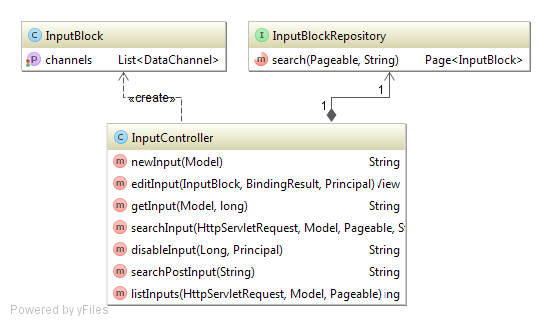
\includegraphics[width=\textwidth, center]{managementInputs}
	\caption{Interacţiunea dintre repository, controller si entitate}
	\label{fig:managementInputs}
\end{figure}

\subsubsection{Managementul blocurilor de intrare}
Pe lângă elementele descrise mai sus, la management-ul blocurilor de intrare trebuie ca utilizatorul sa poată vizualizeze si modifica lista de canale a unui bloc. In vederea implementării acestei particularităţi, in dialogul modal pentru adăugare si modificare a fost realizat un formular dinamic cu cate o line pentru fiecare canal de date. Pentru blocurile de intrare care au deja un canale ataşate, acest formular este generat de către server, in template-ul thymeleaf \code{input.html}, iar, dinamismul formularului este implementata cu ajutorul unor funcţii JavaScript care manipulează structura documentului.
\begin{figure}[H]
	\centering
	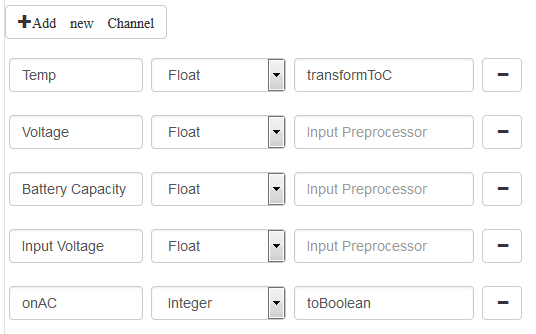
\includegraphics[width=0.8\textwidth, center]{editInput}
	\caption{Formular HTML dinamic pentru editarea canalelor unui bloc de intrare }
	\label{fig:editInput}
\end{figure}
Pentru selectarea blocului de preprocesare a fost folosit endpoint-ul din API de la adresa \code{/blocks/getBlocks} care returnează lista tuturor blocurilor de procesare in format JSON. Aceasta lista este folosita pentru permite completarea automata a câmpului blocul de preprocesare a datelor unui canal, folosind librăria JavaScript \textbf{Bootstrap 3 Typeahead} \autocite{typeahead}.

\subsubsection{Managementul blocurilor de procesare}
O particularitate a editării blocurilor de procesare este folosirea librăriei JavaScript \textbf{CodeMirror}\autocite{codemirror} pentru afişarea codului, cuvintele cheie ale limbajului dat de tipul blocului fiind evidenţiate, acest lucru făcând dezvoltarea codului mult mai facila. Un alt avantaj al acestei librari este posibilitatea găsirii erorilor de sintaxa mult mai rapid, fără a testa blocul. Aceasta funcţionalitate este implementata cu ajutorul unei funcţii care se executa de fiecare dată când valoarea selectată in input-ul "Block Type" se modifică.
\begin{figure}[H]
	\centering
	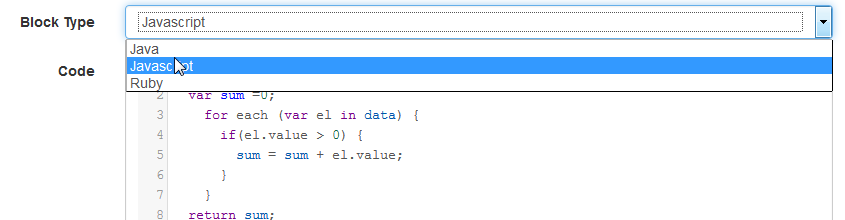
\includegraphics[width=1.2\textwidth, center]{codemirrorExample}
	\caption{Modificarea limbajului din editorul CodeMirror in funcţie de tipul blocului}
	\label{fig:codemirrorExample}
\end{figure}
\subsubsection{Managementul diagramelor}
Pentru implementarea funcţiilor de design vizual al diagramelor funcţionale s-a ales librăria JavaScript \textbf{GoJS} \autocite{gojs}. Aceasta permite implementarea a diagrame interactive, fiind compatibila atât cu toate browsere-le cat si cu dispozitivele mobile moderne. Deoarece asigura suport pentru drag-and-drop, copiere si lipire, undo si redo dar si multe alte funcţionalităţi, librăria reprezinta un punct foarte bun de plecare pentru implementarea diagramelor. Un alt avantaj al acestei librarii este ca suporta adăugarea de condiţii asupra diagramei chiar la construcţia acesteia. Din acest motiv, librăria a fost configurata sa nu permită  decât legături de la o ieşire la o intrare, si canalul de ieşire sa nu poată fi legat decât la o singura ieşire.

In vederea realizării acestor configurări, fişierul JavaScript \code{diagram.js}. Aici sunt configurate tipurile de blocuri:
\begin{itemize}
	\item \textbf{Canale de intrare}: acestea sunt configurate sa nu poată avea intrări, si sa doar o singura ieşire. Atunci când un canal de intrare este selectat, utilizatorul poate sa ii atribuie un nume si sa selecteze care este canalul referfeniţat de acel bloc. Aceasta selecţie se face cu ajutorul unui input cu auto completare.
	\item \textbf{Blocuri de procesare}: deoarece numărul de intrări este variabil, funcţia  \code{addPort} a fost implementata. Aceasta este apelata atunci când utilizatorul da click pe opţiunea "Add input" din meniul contextual al blocului. Pentru operaţiunea de ştergere a portului, funcţia \code{removePort(port)} a fost implementata. Ordinea acestor porturi determina ordinea elementelor din lista cu care este apelat blocul de procesare. Atunci când blocul este selectat, utilizatorul poate sa ii atribuie un nume si sa selecteze care este blocul de procesare referfeniţat de acel bloc. Aceasta selecţie se face cu ajutorul unui input cu auto completare. Astfel, acelaşi bloc de procesare poate fi folosit de mai multe ori in cadrul aceleiaşi diagrame. Pentru uşurinţă dezvoltării, linkuri către detaliile blocului de procesare sunt disponibile chiar in interiorul diagramei.
	\item \textbf{Final}: bloc ce semnifica canalul de ieşire a diagramei. Configurat cu un singur port de intrare, el nu poate fi legat decât la o singura ieşire.
	\item \textbf{Comentariu}: nu se poate lega in diagrama si nu ia parte la execuţia acesteia. 
\end{itemize}
Toate aceste blocuri sunt adăugate si într-o paleta pentru adăugare uşoară in diagrama. Deoarece blocul "Final" nu poate avea decât o singura instanta, acesta nu este disponibil in paleta.
\begin{figure}[H]
	\centering
	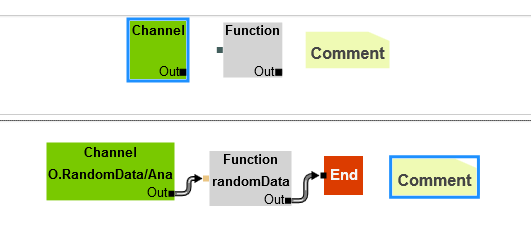
\includegraphics[width=1.2\textwidth, center]{diagramPalleteAndExample}
	\caption{Paleta de blocuri si exemplu de instante ale acestora}
	\label{fig:diagramPalleteAndExample}
\end{figure}
Când utilizatorul salvează o diagrama, un model JSON a acesteia este generat, model ce este apoi salvat in baza de date. In acest model sunt salvate atât proprietăţile diagramei, urmate de o lista nodurilor, si nu in ultimul rând legăturile dintre noduri.

\subsubsection{Administrare tag-uri}
După cum s-a discutat in secţiunea despre securitate, fiecare entitate care este administrata de utilizator poate avea mai multe taguri. Acestea reprezinta o lista de cuvinte care specifica un concept, spre exemplu, toate entităţile care sunt folosite într-o diagrama pot avea acelaşi tag. Tagurile permit astfel gruparea entităţilor, fiind folosite in căutare.
\begin{figure}[H]
	\centering
	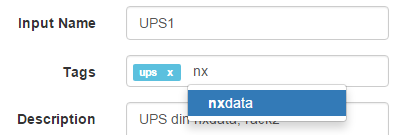
\includegraphics[width=0.7\textwidth, center]{tagsEdit}
	\caption{Editarea tag-urilor unui bloc de intrare}
	\label{fig:tagsEdit}
\end{figure}
Pentru implementare, pe partea de server au fost creata clasa \code{ApplicationTag}, cu doua câmpuri: nume, si Id. Toate instantele acestei clase sunt salvate in baza de date in tabela \code{application\_tag} iar endpoint-ul \code{/tags/getTags} care întoarce toate tag-urile din acea tabela. Acest serviciu API este folosit de librăria JavaScript  Bootstrap Tags Input \autocite{tagsinput}, care, împreună cu librăria de autocompletare \autocite{typeahead} permite utilizatorului sa selecteze taguri deja existente. Atunci când utilizatorul introduce totuşi un tag care nu exista deja in baza de date, acesta este creat automat, fiind setat direct pe entitatea modificata. Fiecare \code{ManagedEntity} are un set de taguri, permiţând salvarea tagurilor in baza de date, într-un tabel separat, care implementeaza relaţia de Multi-la-Multi dintre entitate si \code{ApplicationTag}.
\begin{figure}[H]
	\centering
	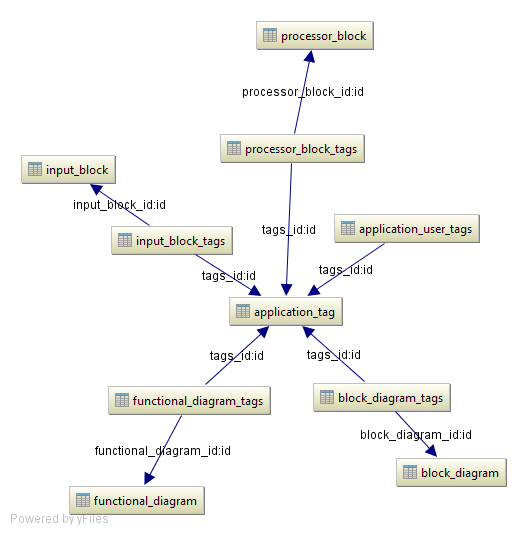
\includegraphics[width=\textwidth, center]{tags}
	\caption{Relaţiile dintre tabela \code{tags} si celelalte entităţi}
	\label{fig:tags}
\end{figure}
\subsection{Monitorizare}
O chestiune de mare importanta este vizualizarea datelor ce au intrat sau au fost procesate de aplicaţie. In acest scop, a fost implementata vizualizarea datelor in timp real. Pentru extragerea informaţiilor de pe un canal se folosesc endpoint-urile din API de la \code{/api/fetch/{channelId}} si , care întorc punctele de pe un canal dintr-un anumit interval de timp, într-un format JSON.

Deoarece datele procesate de aplicaţie sunt de mai multe tipuri, apare totuşi problema modului lor de afişare. In funcţie de datele întoarse prin API, se selectează unul din doua moduri de afişare; Pentru datele numerice a fost aleasa o reprezentare cu ajutorul unui grafic, folosind librăria dygraphs \autocite{dygraphs}, iar pentru datele care nu pot fi reprezentate numeric, acestea sunt afişate tabelar.

Pentru ambele moduri de reprezentare, utilizatorul are opţiunea sa obţină doar datele dintr-o anumita perioada de timp, sau chiar ultimele înregistrări pe acel canal. Acest mod de selecţie este ilustrat in \cref{fig:monitorDataFilter}
\begin{figure}[H]
	\centering
	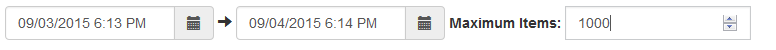
\includegraphics[width=1.2\textwidth, center]{monitorDataFilter}
	\caption{Filtrarea datelor obţinute}
	\label{fig:monitorDataFilter}
\end{figure}
\section{API-ul aplicaţiei}
Pentru a permite interfaţarea aplicaţiei cu alte servicii, dar si pentru a facilita dezvoltarea unor interfeţe web dinamice, aplicaţia dispune de un api REST. Acesta a fost configurat sa folosească date in format JSON.

In următoarea lista sunt descrise toate endpoint-urile API-ului, împreună cu detalii despre folosirea acestora. In afara de câteva excepţii menţionate, toate aceste servicii folosesc metoda HTTP GET.
\begin{itemize}
	\item \code{/blocks/getBlocks}: întoarce toate blocurile de procesare din baza de date. 
	\item \code{/blocks/getChannels}: întoarce toate canalele declarate in baza de date. Pentru fiecare canal returnat, se specifica de la ce bloc de intrare face parte, sau dacă este ieşirea unui diagrame funcţionale.
	\item \code{/tags/getTags}: întoarce toate tagurile existente in aplicaţie.
	\item \code{/api/put/\{inputId\}/\{channelId\}/\{data\}}: Adaugă punctul \code{data} pe canalul specificat prin \code{channelId}. Datele primite sunt in format \code{String}, care respecta standardul specificat in RFC3986 \autocite{rfc3986}. Foloseşte metoda PUT.
	\item \code{/api/put/openTDSB}: Adaugă date in formatul openTDSB\autocite{openTSDB}. In corpul requestului trebuie sa se afle un JSON care respecta standardul impus. Foloseşte metoda PUT.
	\item \code{/api/fetch/\{channelId\}}: Întoarce date de pe canalul \code{channelId}. Următorii parametrii pot fi folosiţi pentru a extrage doar anumite date:
	\begin{itemize}
		\item \code{from}: Data de început a istoricului, in format ISO 8601.
		\item \code{to}: Data de final a istoricului, in format ISO 8601.
		\item \code{maxItems}: Numărul maxim de înregistrări ce sunt returnate. Acest parametru are $500$ ca valoare implicita.
	\end{itemize}
	\item \code{/api/fetch/last/\{channelId\}}: Întoarce date de pe canalul \code{channelId}. Următorii parametrii pot fi folosiţi pentru a extrage doar anumite date:
	\begin{itemize}
		\item \code{maxItems}: Numărul maxim de înregistrări ce sunt returnate. Acest parametru are $500$ ca valoare implicita.
	\end{itemize}
\end{itemize}
Pe lângă aceste metode, aplicaţia mai pune la dispoziţie si API-ul generat automat cu ajutorul Spring Data. Acesta permite adăugarea, modificarea, ştergerea si cutarea entităţilor folosite in aplicaţie programatic.

\section{Executarea unui bloc de procesare}
Blocurile de procesare este folosit Spring Bean-ul \code{BlockExecutor}. Acesta este responsabil de iniţializarea tuturor implementărilor pentru interfaţa \code{GenericBlockExecutor}. Pentru fiecare implementare exista un câmp asociat in enumeraţia \code{ProcessorBlockType}, câmp care este folosit ca proprietate in entitatea \code{ProcessorBlock}. Acest Bean poate fi apoi injectat folosind adnotarea \code{@Autowired} in toate clasele care doresc sa execute blocuri.

Interfaţa \code{GenericBlockExecutor} are o singura metoda \code{processData} cu doi parametrii: unul de tip String, in care este codul funcţiei ce trebuie executat, si unul de tip \code{List<DataPoint>} care conţine toate punctele ce pot fi folosite in blocul respectiv. Clasa \code{DataPoint} au doua câmpuri: valoare si instanta de timp. Următoarele implementări a interfeţei \code{GenericBlockExecutor} exista in sistem:
\begin{itemize}
	\item \code{JavaBlockExecutor}: Acest executor reprezinta un caz special deoarece foloseşte clase locale, ce sa afla deja in classpath-ul JVM-ului pe care rulează aplicaţia. Aceste blocuri pot fi folosite pentru a extinde aplicaţia cu cod de înaltă performaţă, acţionând ca un mecanism de extensii ale aplicatei, permiţând interacţiunea cu alte sisteme. Aceste blocuri pot sa reprezinte doar o interfaţa pentru apelul unor librarii externe, făcând posibila, spre exemplu, implementarea unui bloc care sa execute scripturi MATLAB.
	Acest bloc primeşte ca parametru doar numele canonic al clasei, iar, la execuţie încarcă clasa referentiata folosind funcţii din pachetul \code{java.lang.reflect}. Dacă clasa nu este găsită, sau o eroare are loc la execuţia clasei, o excepţie de tipul \code{BlockExecutionException} este generată.
	\begin{figure}[H]
		\centering
		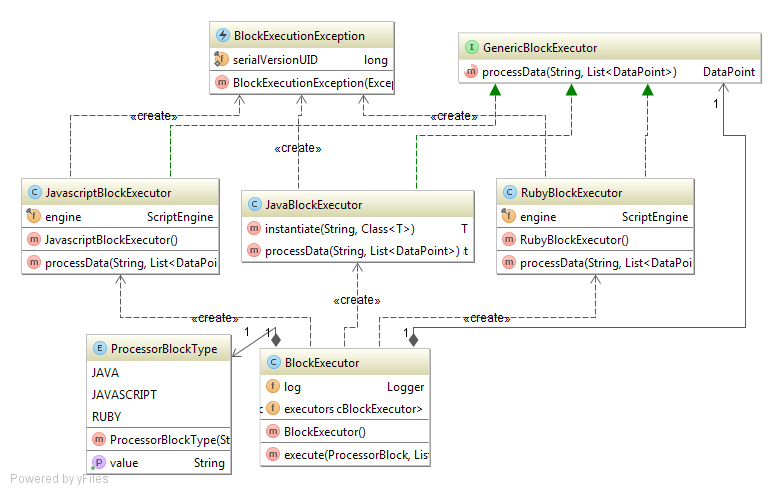
\includegraphics[width=1.3\textwidth, center]{blockExecutors}
		\caption{Clasele ce asigura executarea unei diagrame}
		\label{fig:blockExecutors}
	\end{figure}
	\item \code{JavascriptBlockExecutor}: Executor ce poate rula cod JavaScript pe server. Aceste blocuri trebuie sa conţină o funcţie \code{parseInput} care ia ca parametru o lista de \code{DataPoint}. Pentru execuţia blocurilor de acest tip, standardul JSR 223 \autocite{JSR223} vine in ajutor prin abstractizarea funcţionalităţii interne necesare execuţiei de cod scris într-un limbaj dinamic, direct in maşina virtuala Java. In versiunea 8 a JVM-ului aceste funcţii sunt executate folosind runtime-ul de înaltă performanta Nashorn, care este accelerat de modificări recente, introduse in JSR 292  \autocite{JSR292}, ridicând performanta codului JavaScript la un nivela apropiat de funcţiile scrise in Java. Pentru versiunile precedente de JVM este folosit Mozilla Rhino. Dacă funcţia \code{parseInput}  nu este găsită, sau o eroare are loc la execuţia script-ului, o excepţie de tipul \code{BlockExecutionException} este generată. Scriptul poate returna direct instante ale interfeţei \code{DataPoint}, sau alte obiecte care sunt apoi reprezentate ca un \code{StringDataPoint}.
	
	\item \code{RubyBlockExecutor}: Executor ce rulează cod Ruby pe server. Din punct de vedere al implementării este similar cu \code{JavascriptBlockExecutor}, însă foloseşte librăria JRuby \autocite{jruby} .
	
\end{itemize}

\section{Executarea unei diagrame funcţionale}
Pentru execuţia diagramelor este folosit Spring Bean-ul \code{DiagramExecutor}. Acesta este responsabil atât de parsarea unei diagrame cat si de execuţia si extragerea rezultatelor. Acest Bean poate fi apoi injectat folosind adnotarea \code{@Autowired} in toate clasele care doresc sa execute diagrame.

Parsarea este realizata cu ajutorul interfeţei \code{DiagramParser}, aceasta permiţând transformarea diagramei într-un graf reprezentat printr-o lista de adiacenţă. O implementarea a acestei interfeţe este clasa \code{GoJsDiagramParser} care parsează JSON-ul general de librăria GoJS. Aceasta parsare se face cu ajutorul librăriei Jackson, folosind schema din figura \cref{fig:gojsdiagramModel}. Dacă parsarea nu este realizata cu succes, atunci o excepţie de tipul \code{DiagramParseException} este aruncată.
Dacă se doreşte înlocuirea librăriei de front-end pentru realizarea diagramelor, sistemul poate fi adaptat doar prin scrierea unei noi clase care implementează \code{DiagramParser}.

\begin{figure}[H]
	\centering
	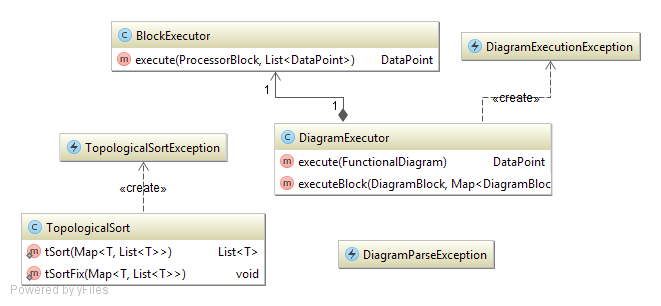
\includegraphics[width=\textwidth, center]{diagramExecuteClasses}
	\caption{Clasele implicate in executarea unei diagrame}
	\label{fig:diagramExecuteClasses}
\end{figure}
Odată ce parsarea a fost efectuata, execuţia blocului poate continua: folosind clasa \code{TopologicalSort}, o implementare a \cref{alg:khan} cu tipuri generice si expresii lambda, este executata. Apoi, \cref{alg:executeDiagram} este executat, si, cu ajutorul bean-ului \code{BlockExecutor} blocurile din diagrama sunt executate. Rezultatul final al metodei \code{execute} este un \code{DataPoint} care va fi salvat in baza de date, pe canalul de ieşire a diagramei.

O alta chestiune importantă este determinarea momentelor când o diagrama trebuie executată. In acest scop, pe fiecare canal are un set de diagrame care trebuie lansate atunci când se primesc informaţii noi. Aceasta lista este actualizată de fiecare data când diagrama se modifica prin interfaţa web. Metodele din \code{DiagramParser} folosite pentru a obţine lista de canale utilizate si pe fiecare dintre acestea, pe proprietatea \code{Set<FunctionalDiagram> subscribedDiagrams} este adăugată acea diagrama. Pentru a nu se pierde consitenţa datelor, cat timp diagrama este modificata, ea nu se mai poate lansa in execuţie.
\begin{figure}[H]
	\centering
	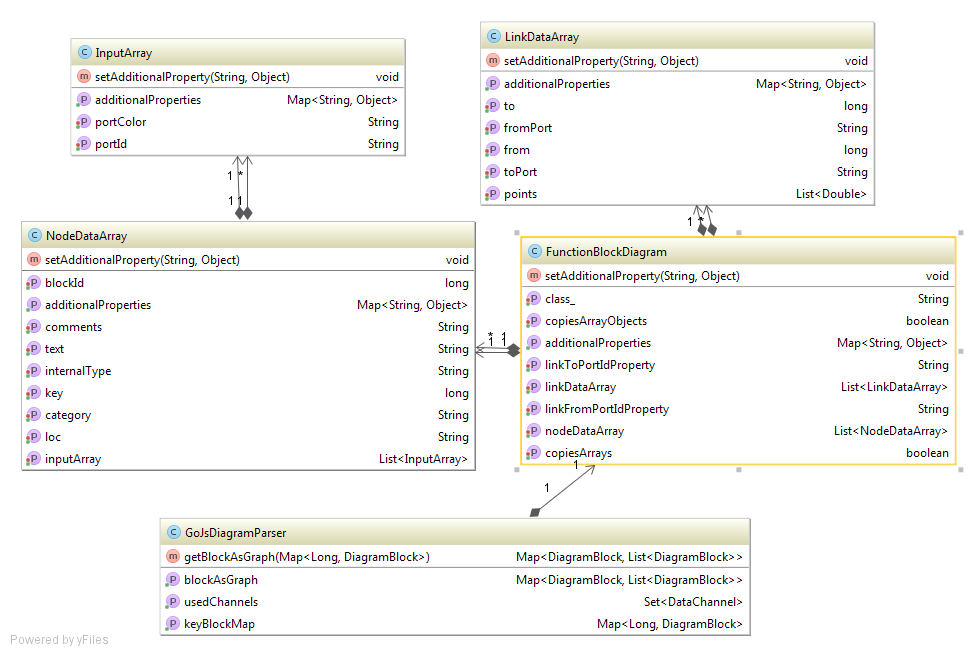
\includegraphics[width=1.2\textwidth, center]{gojsdiagramModel}
	\caption{Modelul de date pentru diagramele GoJS}
	\label{fig:gojsdiagramModel}
\end{figure}
\section{Serviciul de date}
Serviciul de date, implementat prin Spring Bean-ul \code{DataService} permite abstractizarea modului in care \code{DataPoint}-urile sunt scrise in baza de date. In aceasta implementare, datele sunt stocate in aceeaşi instanta de PostgreSQL ca si entităţile.
\begin{figure}[H]
	\centering
	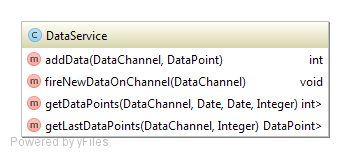
\includegraphics[width=0.6\textwidth, center]{dataService}
	\caption{Interfaţa aplicaţiei cu baza de date pentru informaţii}
	\label{fig:dataService}
\end{figure}
Aceasta clasa asigura si execuţia diagramelor din lista de \code{subscribedDiagrams} a canalului ce primeşte date. Aceasta execuţie se executa in mod \textbf{asincron}, pentru a nu bloca firul de execuţie care primeşte date. Asincornicitatea este implementata printr-un pool de thread-uri care primesc task-uri de execuţie, thread-ul apelant nefiind interesat de rezultatul execuţiei. Astfel, putem considera ca implementarea pe mai multe fire de execuţie este de tipul fire-and-forget.
\section{Baza de date}